\section{Data generation for the sphere}
What turned out to be quite challenging in this project was to have data of good quality for training data-driven methods on a sphere.
Hence, we have investigated several approaches to generate data for the sphere.
Both investigated the possibility of generation data ourselves and utilizing external data sources.


\subsection*{Projecting 2D data to the sphere}
Our first approach was to project the solution data from the 2D SWE to the sphere.
To generate high quality data we set the CFL number to 0.8, for ensuring stability.
We treat $\theta$ and $\phi$ as we have treated $x$ and $y$ in the 2D case.
We set the number of grid points in the theta direction af $N_{theta} = 200$ and the number of grid points in the phi direction as $N_{phi} = 100$.
The reason for the double number in the theta direction is that distance is double the distance in the phi direction.
The results are shown in~\autoref{fig:sphere_projected_water_height_timesteps}.
\begin{figure}[H]
    \centering
    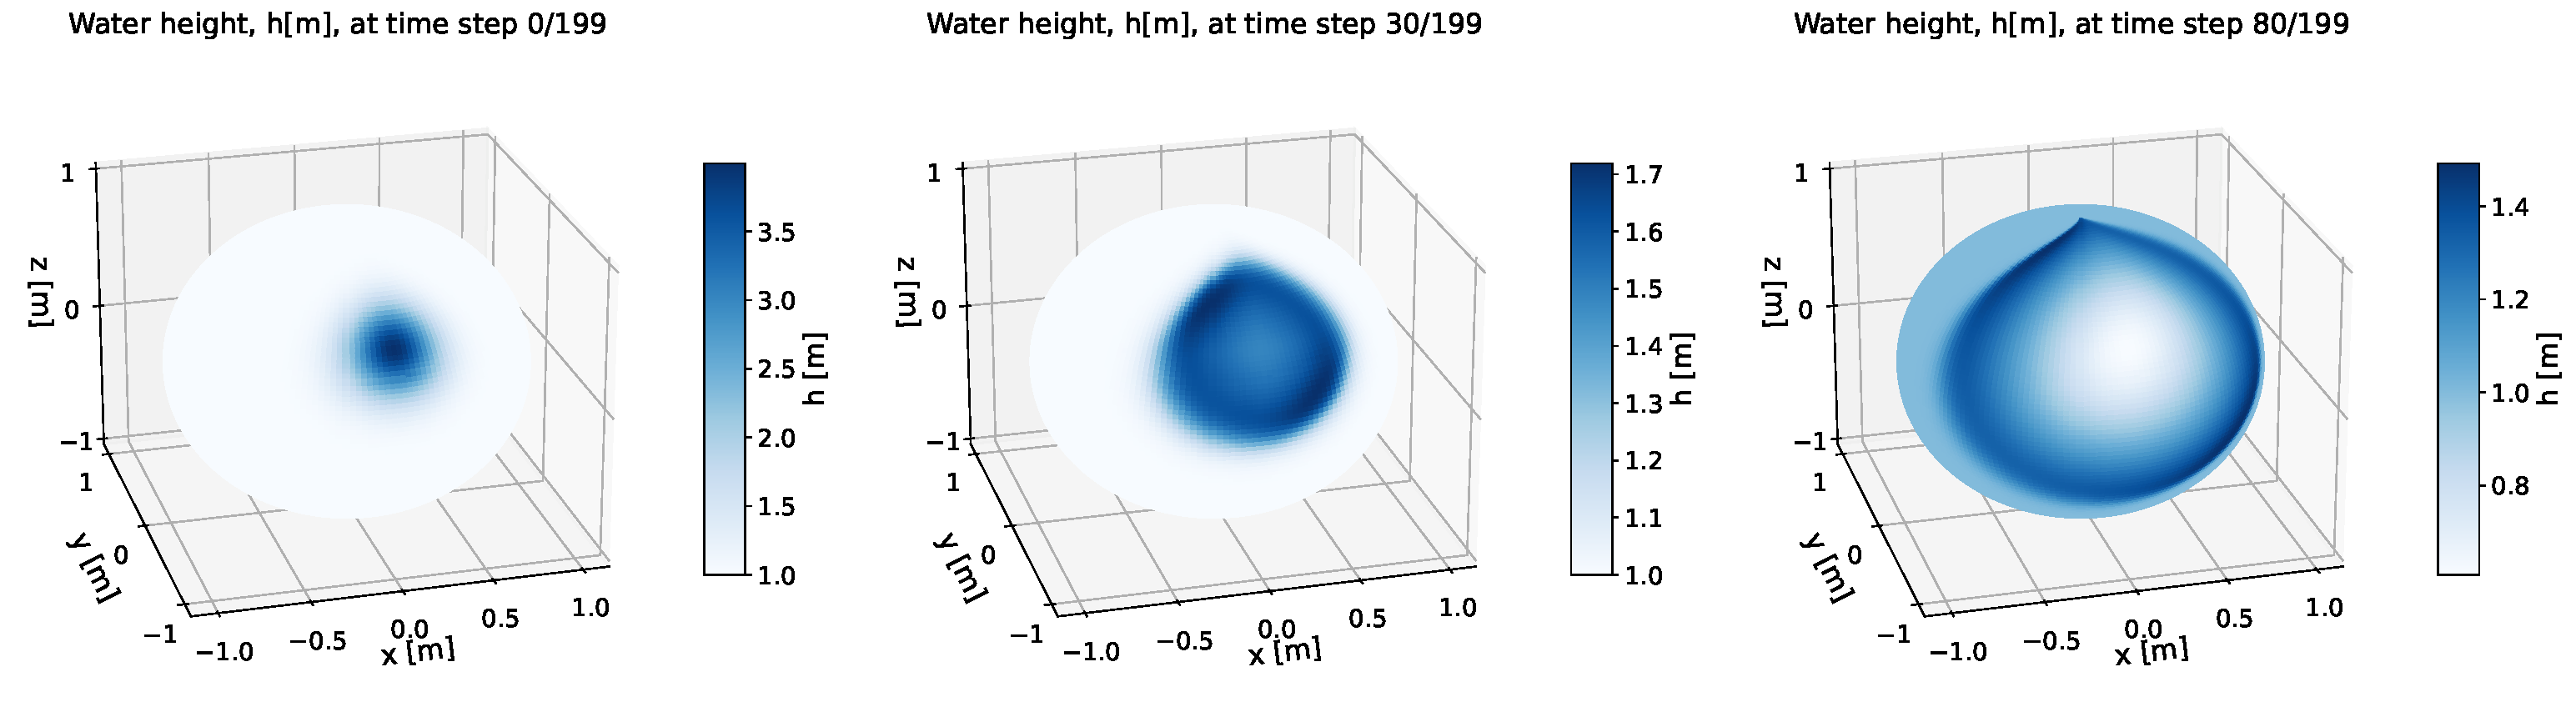
\includegraphics[width=0.95\textwidth]{C:/Users/Matteo/Shallow-Water-Equations/plots/sphere_projected_water_height_timesteps.pdf}
    \caption{Water height on the sphere for different timesteps.}\label{fig:sphere_projected_water_height_timesteps}
\end{figure}
In~\autoref{fig:sphere_projected_water_height_timesteps} we see how the water height evolves over time on the sphere.
We see the initial Gaussian bump, which is then propagating over the sphere.
As we see there are some singularities esoecially at the poles.
This is among other things due to the fact that we are not taking the curvature of the sphere into account.
For some applications, this approach may be acceptable. 
Consider the case, where we consider a small region around the equator, then the projection will be quite accurate.
However, for this project, we want to consider the whole sphere, and hence we need to consider the curvature of the sphere.
Therefore we can not use this data.

\subsection*{Mesh generation for the sphere}
To solve the SWE on the sphere, we must use another grid, than the regular grid used in the 2D case.
Hence, we use the icosahedral grid, which is a grid that approximates the sphere with triangles.
The grid can be generated in different generations, depending on the level of detail we need. 
For each time we refine to a higher level, the number of triangles increases by a factor of four, i.e., we split each triangle into four smaller triangles.
Meaning that the number of triangles is increasing drastically with each level of refinement.
The grid is generated by the Github: https://github.com/siddharth-maddali/SphereMesh/tree/master and then rewritten to Python.
The grid for the first 4 levels of refinement is shown in Figure~\ref{fig:icosahedral_grid}.
\begin{figure}[H]
    \centering
    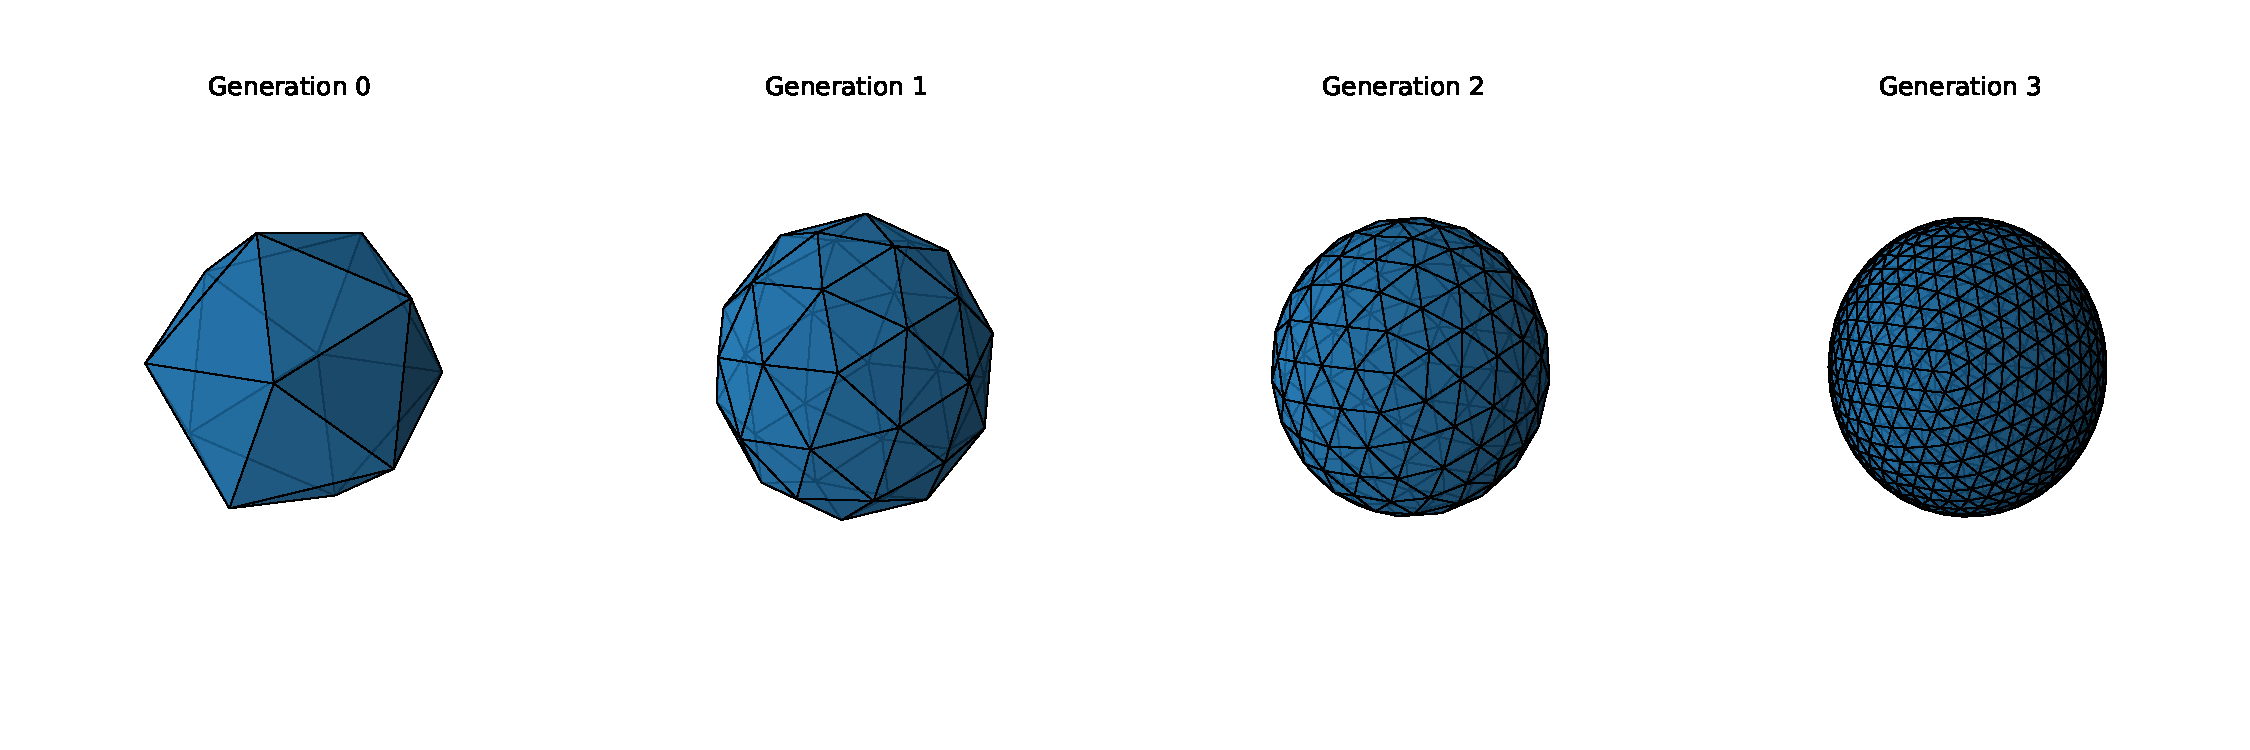
\includegraphics[width=\textwidth]{C:/Users/Matteo/Shallow-Water-Equations/plots/icosahedral_mesh_refinement.pdf}
    \caption{Icosahedral grid for the first 4 levels of refinement.}\label{fig:icosahedral_grid}
\end{figure}
For simplicity, we will begin by considering the first level of refinement, which consists of 20 triangles.
The matrix tri is a $20 \times 3$ matrix, where each row represents a triangle and the three columns represent the three vertices of the triangle.
The vertices are stored in the matrix $P$, which is a $12 \times 3$ matrix, where each row represents a vertex and the three columns represent the x, y, and z coordinates of the vertex.
The vertices are normalized to the unit sphere, i.e., the radius of the sphere is 1.
The idea is now, that similar to the case in cartesian coordinates, we loop through each cell, in this case triangles, and calculate the fluxes between the cells.
We must be aware of which cells/triangles are neighbors, and we must also be aware of the orientation of the triangles, i.e., the normal vector of the triangle.
The normal vector is calculated by the cross product of the two vectors that span the triangle.
The normal vector is then normalized to the unit sphere.
The matrix tri is my Element to Vertex matrix. 
I also need an Element-to-Face table and a Element-to-Element table.
The Element-to-Face table is used to define which edges or faces belong to each triangle.
Each face of a triangle is an edge shared between two triangles.
The Element-to-Element table is used to define which triangles are neighbors. 
That is, it indicates which triangles share an edge. This is important when calculating the fluxes between the triangles.
To construct this table we loop through each triangle and check if the edge of the triangle is shared with another triangle.


We make the FVM to solve SWE for a triangular grid on the sphere.
For each triangle, we consider each face (edge).
For each face we define the normal vector in terms of the spherical unit vectors $\mathbf{e}_\theta$ and $\mathbf{e}_\phi$.
The spherical unit vectors at a point are:
\begin{align*}
    \mathbf{e}_\theta &= \begin{bmatrix}
        - \sin(\theta) \\
        \cos(\theta) \\
        0
    \end{bmatrix}, \\
    \mathbf{e}_\phi &= \begin{bmatrix}
        \cos(\phi) \cos(\theta) \\
        \cos(\phi) \sin(\theta) \\
        -\sin(\phi)
    \end{bmatrix}.
\end{align*}
Where $\mathbf{e}_r$ is the radial direction, going outward from the origin.
$\mathbf{e}_\theta$ is the longitude direction, and $\mathbf{e}_\phi$ is the latitude direction.
The unit vectors are tangensial to the sphere.
We do not need to consider the radial direction, as the SWE is only in the tangential directions.

Now we have the cartesian edge vectors in tangential directions, $\mathbf{e}_0, \mathbf{e}_1, \mathbf{e}_2$.

The projection of an edge vector \( \mathbf{e}_i = (e_{ix}, e_{iy}, e_{iz}) \) onto \( \mathbf{e}_\theta \) is:

\[
\mathbf{e}_i \cdot \mathbf{e}_\theta = e_{ix} \left( -\sin \theta \cos \phi \right) + e_{iy} \left( -\sin \theta \sin \phi \right) + e_{iz} \cos \theta
\]

Similarly, the projection onto \( \mathbf{e}_\phi \) is:

\[
\mathbf{e}_i \cdot \mathbf{e}_\phi = e_{ix} \left( -\sin \phi \right) + e_{iy} \cos \phi
\]

Recall that the cross product between two vectors in 3D produces a third vector that is orthogonal to the two input vectors, i.e., the plane spanned by the two input vectors.

For a given face $f$ of a triangle, we first calculate the Cartesian face normal $\mathbf{n}_f$ as the cross product of the two vectors that span the face.
For a given face $f$ of a triangle, we define the normal vector $\mathbf{n}_f$ is decomposed into the spherical unit vectors as



\subsection*{External data sources}


\begin{figure}[H]
    \centering
    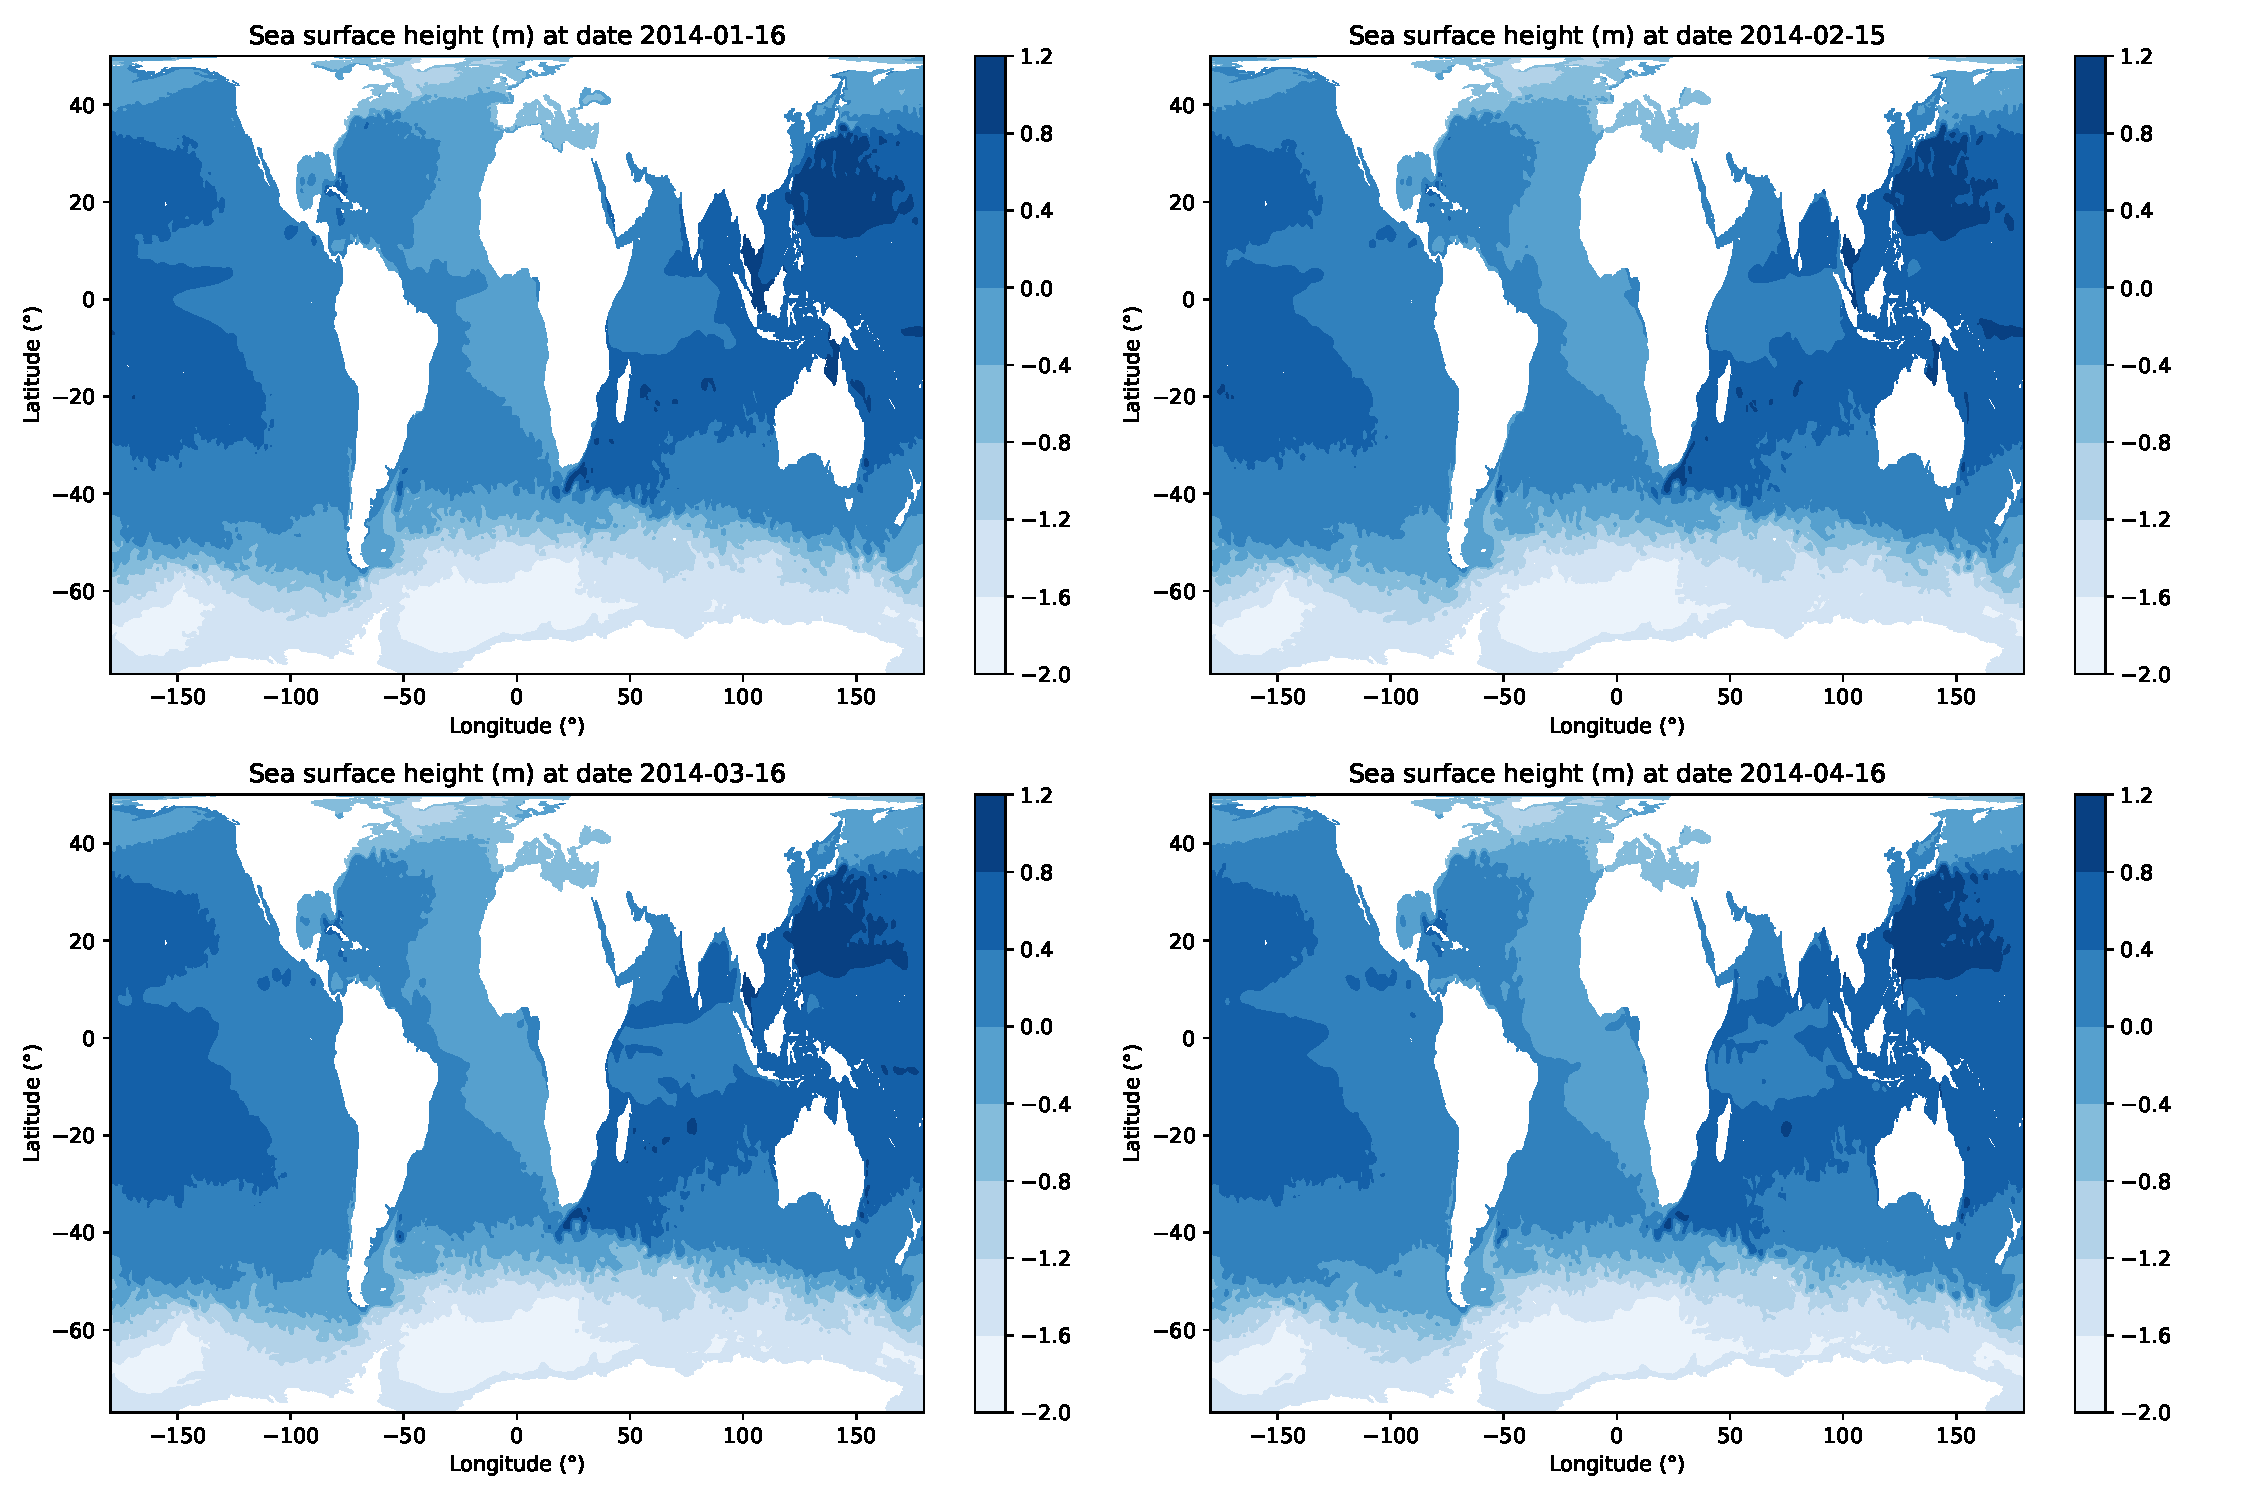
\includegraphics[width=0.95\textwidth]{C:/Users/Matteo/Shallow-Water-Equations/plots/ssh_field.pdf}
    \caption{Sea surface height as the diffference from reference sea surface height for the months Jan-Apr 2014.}\label{fig:copernices-ssh}
\end{figure}


